\chapter{Sistemas de Información Geográficas}

\section{Elementos de cartografía}
\subsection{Definición}
La geodesía es la ciencia que se ocupa de la determinación de la dimensión y forma de la tierra, de la ubicación de posiciones sobre la tierra y la determinación de su campo gravitacional. La geodesia puede subdividirse en geodesia geométrica, geodesia fisica, y geodesia satelital. La descripción de localizaciones en término geométrico usando sistemas de coordenadas es la principal función de la geodesia geométrica. La medición de la magnitud y dirección del campo gravitacional de la tierra necesaria para el establecimiento de las alturas geoidal y elipsoidal constituye la actividad de la geodesia física. La obtención de datos para varias aplicaciones geodésicas a partir de satélites orbitando la tierra es la función de la geodesia satelital. Los datos geodésicos incluyen una red de puntos caracterizados por su localización y posición La posición consiste en un par o triplete de números llamado coordenadas Lat localización es un lugar del mundo real cuya ubicación espacial se describe por una

posición. Hasta poco la geodesia estaba desconocida por la mayoría de la gente, incluso poca gente habia oido la palabra geodesia. El geodesta habia trabajado silenciosamente en la sombra del topografo hasta el final de siglo recién pasado que vió el nacimiento y resurgimiento de dos grandes tecnologias, el Sistema de Información Geográfica (SIG) y el Sistema Global de Navegacion Satelital (GNSS).

\subsection{Elemento de Geodesia geométrica}

\begin{definition}[Distancia]
    Las distancias son fundamentales en cartogratia y SIG. El término general de distancia significa la longitud de un segmento de curva. Una distancia lineal es la longitud de un segmento de una linea recta. Del mismo modo se ha definido distancia terrestre que se mide sobre la superfiie fisica terrestre usando cadenas. cintas, alambres o ruedas calibradas con odometros: también podria ser estimada sobre un modelo digital de terreno (DTM) como es el caso de una red triangulada irregular (TIN)    
\end{definition}

En realidad la distancia terrestre corresponde a la longitud de un arco. Si $d$ es la longitud del arco $AB$. y $d_0$ su estimador aproximado, entonces $d\approx d_o = \left(dx^2+dy^2\right)^{0.5}$ Una mejor aproximación de $d$ se obtiene subdividiendo el arco $AB$ en tres segmentos de arco, $d_1, d_2$ y $d_3$. de modo que $d\approx d_1+d_2+d_3$ (Fig \ref{sig1}). Si se subdivide $d$ en mus segmentos de arco de taimimios muchos menores hasta que el numero de seguientos de curvas suavizadas tiende al infinito, es decir que la suma de las longitudes de los segmentos tiende a acercarse a d, En este momento el tamaño de los segmentos tiende a acercarse a $d=\sum d_i$. EN este momento el tamaño de los segmentos
\begin{equation}
    d =\int_a \sigma\,d
\end{equation}
\begin{figure}[h!]
\centering
  \includegraphics[width=0.5\textwidth]{sig1.pdf}
  \caption{Si el arco AB es un arco circular, es decir los puntos A y B se localizan sobre un círculo como se muestra}
  \label{sig1}
\end{figure}
La ecuación se transforma en:
\begin{equation}
    d = r\theta
\end{equation}
Una lpinea horizontal se define como la distancia de una línea recta dentro de un plano horizontal, y la línea vertical es la distancai de la línea recta perpendicular al plano local horizontal.

\subsection{Definición de cartografía}
La palabra cartografia proviene del griego GRAPHEIN (escribir o describir) y del latino CHARTA (papel) y cartografia es la descripción o representación del espacio geográfico sobre un papel. El diccionario Multilingual de los términos técnicos define a la cartografia como: "El arte, ciencia y tecnologia de preparación de cartas y el estudio de los mismos tanto como documentos cientificos como de trabajos de arte." Desde este enfoque, los cartas pueden ser considerados como incluyendo todos tipos de planos, cartas, y modelos tridimensionales de porciones o todo el globo terráqueo y cualquier otro cuerpo celestre, a alguna escala.

La cartografia en su significado más general es la ciencia que tiene por objetivo el establecimiento y uso de los mapas: incluye a la Geodesia, determinación geométrica sobre el elipsoide de un número de puntos de apoyos terrestres, y la topografia que es la representación gráfica de detalles del terreno sobre el papel.

Una fotografia muestra todos los objetos dentro de su vista, Un mapa es una abstraccion de la realidad.

El cartógrafo selecciona solamente la información que es esencial para cumplir con el propósito del mapa y de la escala del mapa.

Los Mapas usan simbolos tales como puntos, lineas, patrones de área y colores para transmitir la informacion.

\subsubsection{Uso de los mapas}
\begin{enumerate}
    \item Para localizar sitios o lugares en la superficie terrestre
    \item Para mostrar los patrones de distribucion, y 
    \item Para descubrir las interrelaciones entre diferentes fenómenos mediante el análisis de la información del mapa.
\end{enumerate}

\subsubsection{Escala de los mapas}
\begin{definition}[Escala]
    Es la relación entre el tamaño en el mapa y el tamaño correspondiente sobre el terreno.
\end{definition}

Algunos ejemplos de escalas 1:1, 1:200, 1:20,000, 1:50,000. 1:250,000 etc. Mayor el el denominackor más pequeña sera la escala

Tipo de mapas según la escala:
\begin{itemize}
    \item \textbf{Un mapa con escala grande} muestra una superficie pequeña con mucho detalle: Ej. Escalas mayores que 1:25,000 mapas muy detallados
    \item \textbf{Un mapa con escala pequeña} muestra poco detalle en una grande superficie. Ej. Escalas mentre o igual que 1:500,000. Mapas de reconocimiento y mapas de síntesis o esquemáticos
\end{itemize}

Tipos de mapa según el temario:
\begin{itemize}
    \item Mapas generales (catastrales o topográficos)
    \item Mapas temáticos (Geológicos, de suelos o vegetación)
\end{itemize}

\subsection{Cartografía matemática}

\subsubsection{Sistema de coordenadas}

El objetivo de este tema es proporcionar una breve descripción de los Sistemas locales y globales para lograr un posicionamiento preciso en localización de puntos en el espacio, lo cual es usado en los GPS, en Navegación, y en los Sistemas de Información Geográfica.

Existen varios Sistemas de coordenadas diferentes, basados en una variedad de datum geodésico, unidades, proyecciones, y sistemas de referencia en uso actualmente.
Si se habla sobre coordenadas planares o cartesianas, se determinan los ejes bidimensionales y tridimensionales y esto puede ser consultado con más detalle en el capitulo de Topografía Aplicada de la presente obra.

\subsubsection{Introducción a los datums geodésicos}

El Geoide es una superficie equipotencial relativos al sistema de coordenadas usados para el control geodésico, para el calculo de las coordenadas de puntos sobre la tierra.

Estos constantes incluyen al punto fundamental donde el elipsoide y el geoide coinciden
Cada datum incluye también los parámetros del elipsoide.
El ``fundamental'' que es el punto donde el Geoide y el Elipsoide coinciden se describe a través de sus coordenadas y la orientación de la dirección que une el punto fundamental con el origen de la tierra, y sus valores de desviación Eta y Xi: es la desviación en el meridiano
Eta: es la desviación en la vertical

La desviación de la vertical (Eta) se debe al no coincidir la vertical el Geoide con la vertical en el Elipsoide. Debido al anterior, al realizar la medición de la latitud, no pasa por el origen de los ejes (0,0,0) originando un punto ficticio P' que podría no estar situado sobre el eje de los polos (N-S) generando la desviación en el meridiano. Si el punto P' está situado sobre el eje N-S, entonces la desviación sobre el meridiano es nula.

\subsubsection{Superficie topográfica de la tierra}
Desde los tiempos antiguos ya se sabía que la tierra tenia la forma de una esfera. La Superficie  topográfica de la Tierra es irregular y temporal, además hay variaciones gravitacionales locales, causadas por variación en la composición de la superficie y de la corteza terrestre.  

\textbf{Geoide}
El Geoide es una superficie equipotencial, que se aproxima al nivel medio de los mares prolongado de bajo de los continentes. Todos los puntos sobre el Geoide tiene la misma gravedad. La superficie del Geoide no es uniforme, presenta irregularidades debido a diferente composición mineralógica del interior de la tierra, y también diferente densidad. Eso tiene  como consecuencia que los diferentes puntos sobre el elipsoide están situados a diferentes alturas del centro de la masa de la tierra.

\textbf{Elipsoide}
La superficie matemática que más se aproxima al geoide es el elipsoide de revolución, aplastado en los dos polos. Los parámetros del elipsoide se definen en base a los radios ecuatorial a, el radio polar b, el achatamiento 1/f, y los valores de excentricidad. Estos parámetros difieren según el datum de la figura \ref{sig3}

\begin{figure}[h!]
\centering
  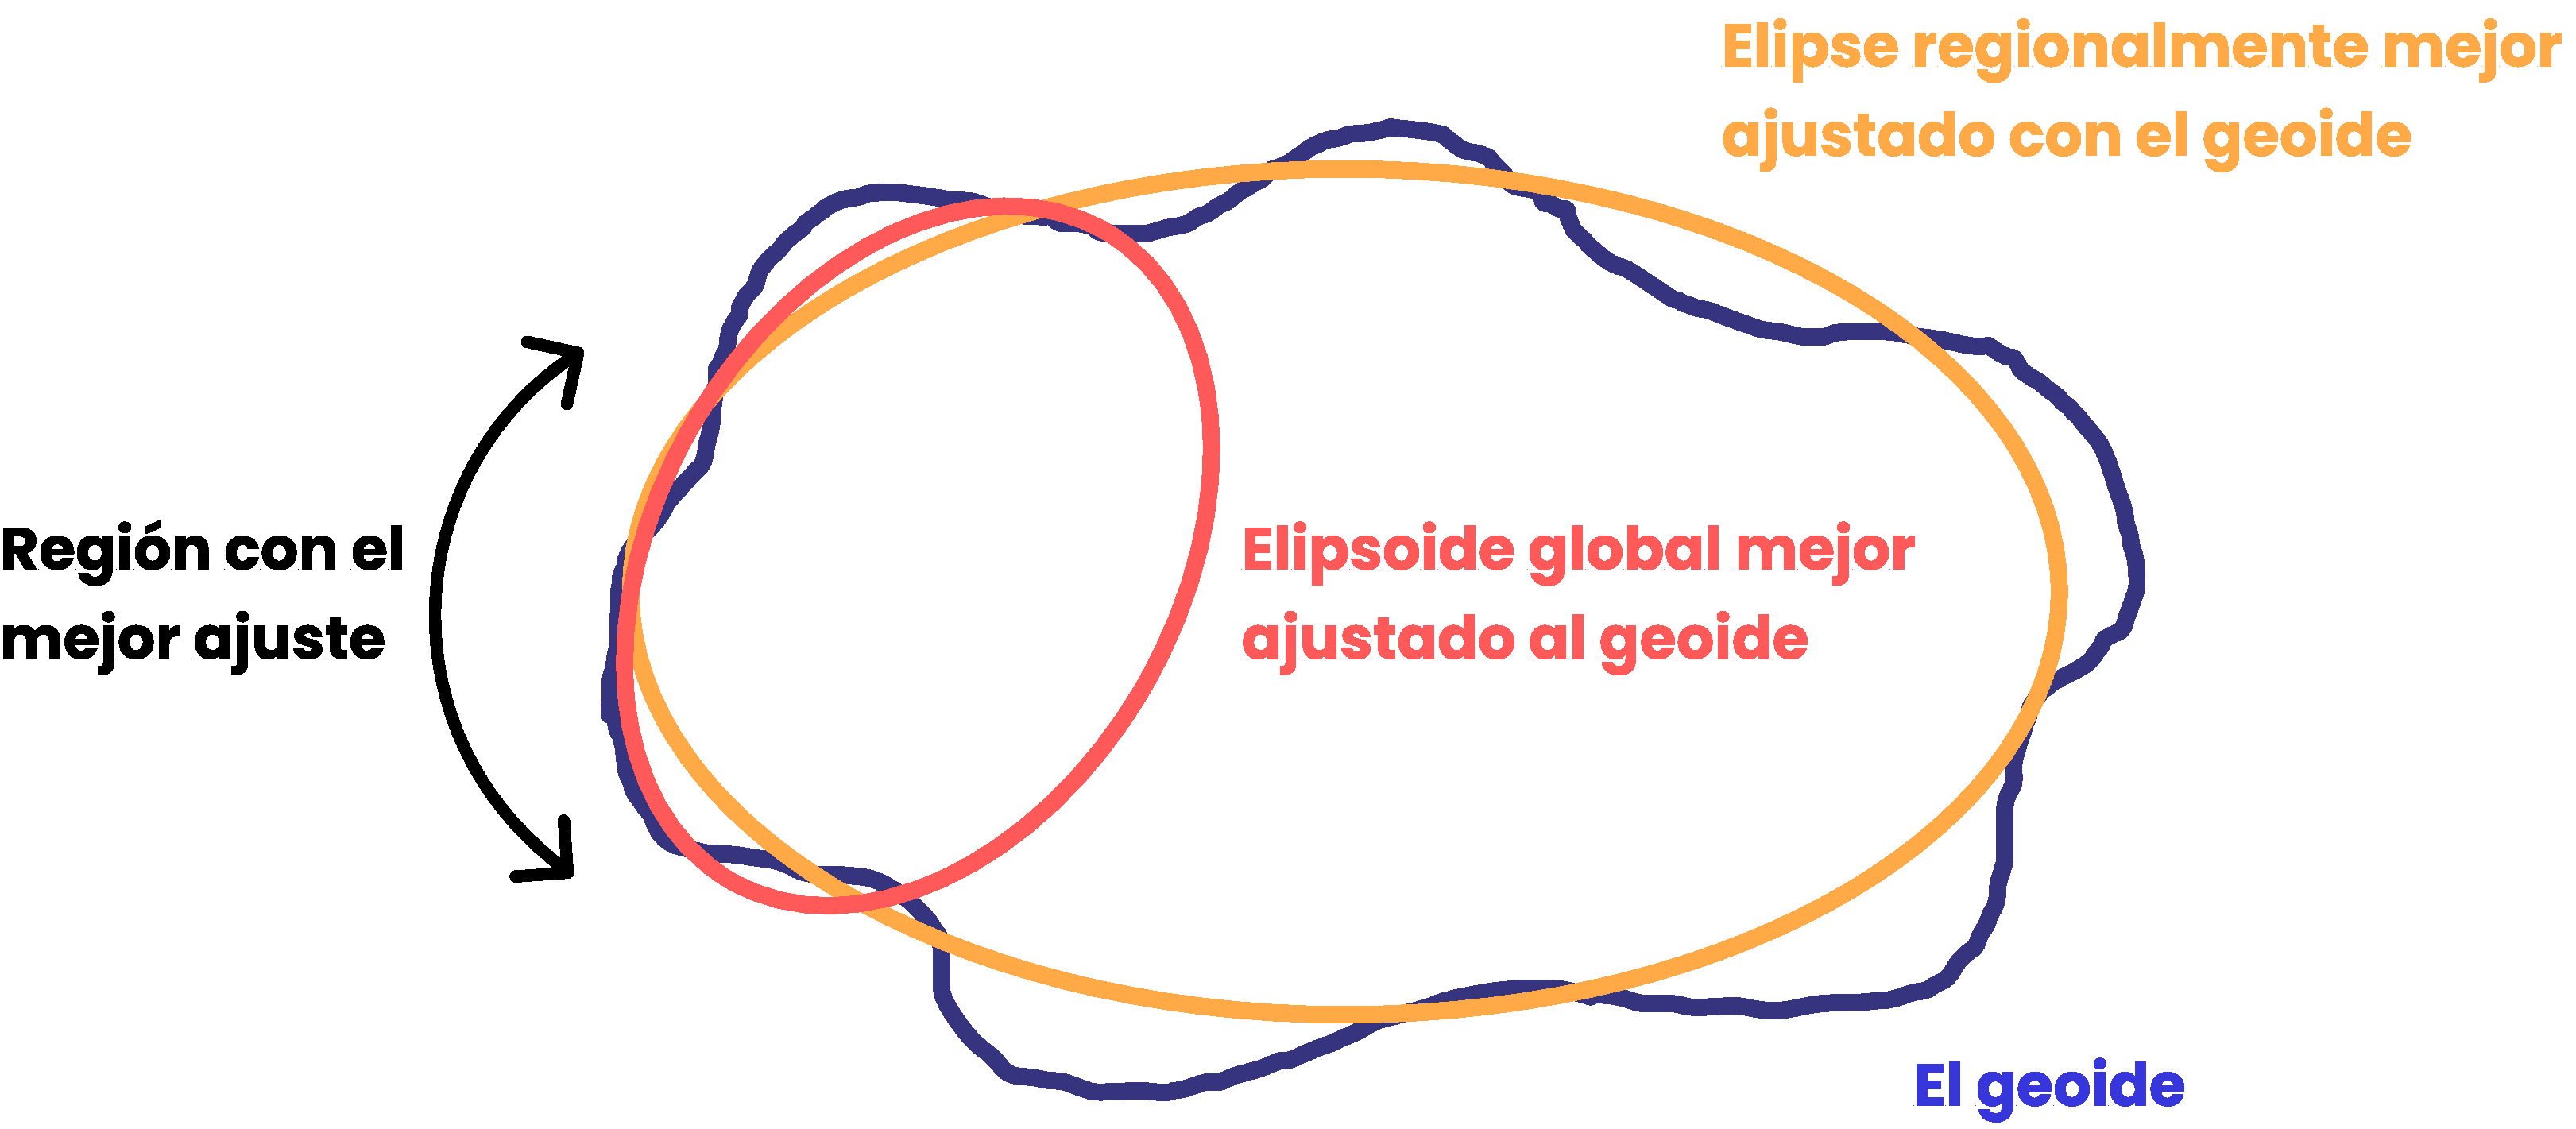
\includegraphics[width=0.5\textwidth]{sig3.pdf}
  \caption{Modelo geoide-elipsoidal de la forma de la Tierra}
  \label{sig3}
\end{figure}
\begin{table}[h!]
\centering
  \begin{tabular}{@{}cc@{}}
  \toprule
  Parámetros                        & Significado                                    \\ \midrule
  a:                                & Semi-eje mayor de la tierra (radio ecuatorial) \\
  b:                                & Semi-eje menor de la tierra (radio polar)      \\
  $f = \frac{a - b}{a}$             & Aplastamiento (achatamiento)                   \\
  $e^2 = \frac{a^2 -b^2}{a^2}$      & Primera excentricidad cuadrada                 \\
  $e_2^{2} = \frac{a^2 - b^2}{b^2}$ & Segunda excentricidad cuadrada                 \\ \bottomrule
  \end{tabular}
  \caption{Parámetros del elipsoide}
  \label{tabsig1}
  \end{table}
  La relación que existe entre estas tres formas de la tierra se muestra en la figura \ref{sig4}.

  La figura \ref{sig4} muestra los diferentes tipos de alturas (ortometrica H, elipsoidal h) y la ondulación geoidal N.
  \begin{figure}[h!]
  \centering
    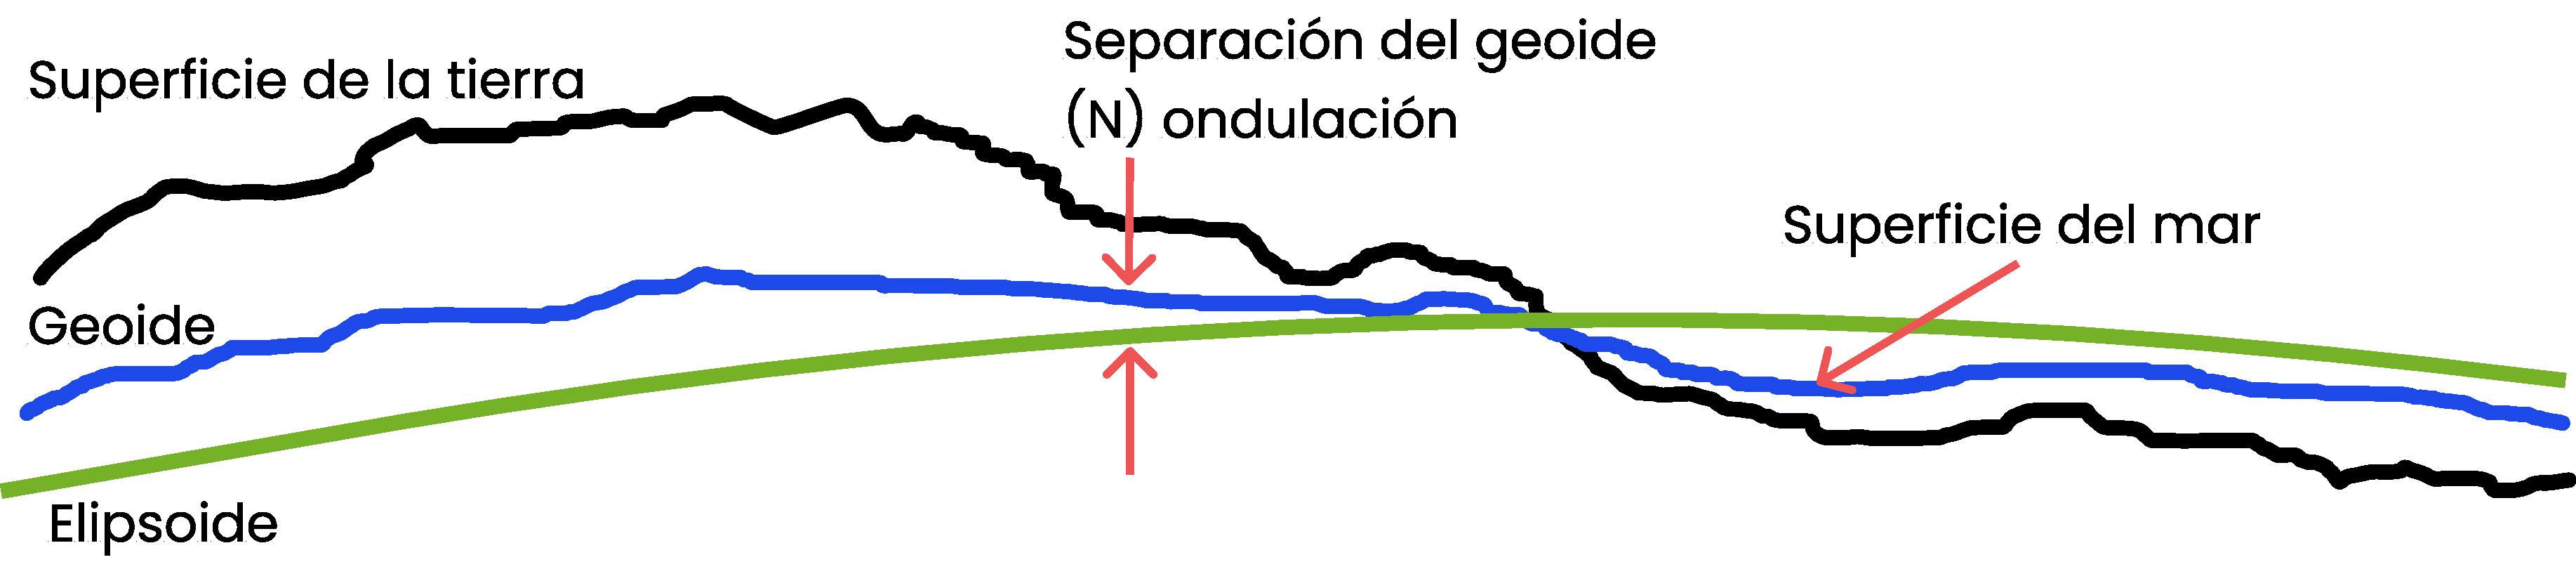
\includegraphics[width=0.5\textwidth]{sig4.pdf}
    \caption{Relación entre Geoide y Elipsoide, y Medición de las alturas elipsoidales h y ortométrica H}
    \label{sig4}
  \end{figure}

\subsection{Coordenadas Geográficas}
\subsubsection{Sistemas de coordenadas globales: Latitudes, longitudes y altitudes}
El sistema de coordenadas geográficas que permite localizar un punto en la superficie del globo es constituido por una red de líneas ortogonales de referencia llamadas paralela y meridiana (Fig.8).  La línea que une a los dos polos corresponde al eje de rotación de la tierra; los extremos de este eje se llaman Polo Norte (PN) y Polo Sur (PS).

Los meridianos consisten de un número infinito de líneas circulares sobre la superficie de la tierra y que pasan por los dos polos, el Polo Norte y el Polo Sur. El primer meridiano denominado meridiano $0^{\circ}$ constituye el origen para la localización hacia el Este o el Oeste esta línea cero de cualquier punto. El primer meridiano, conocido como meridiano Greenwich, divide la tierra en dos zonas: la zona situada al Oeste (W) del meridiano 0 hasta el antimeridiano, y la zona situada al Este (E) del meridiano 0 hasta el antimeridiano. La separación angular del plano meridiano de un punto situado sobre el globo con respecto al plano del meridiano cero es llamado longitud. En la figura 9B, la longitud corresponde al ángulo $\lambda$. El ecuador y los meridianos son divididos en $360^{\circ}$ (grados). La división hexagésimal:
\begin{itemize}
  \item $1^{\circ}$= 60 minutos $(60^{\prime})$
  \item $1^{\prime}$= 60 segundos $(60^{\prime\prime})$
  \item q rotación de la tierra = $360^{\circ}$ = 24 horas
\end{itemize}
Los valores de la longitud varían de 0 a $180^{\circ}$ ($0-180^{\circ}$ E, y $180-0^{\circ}$ W).

Los paralelos son definidos como las líneas de intersección de los infinitos planos perpendiculares al eje de los polos, siendo el Ecuador el paralelo de máximo diámetro (Fig. \ref{sig5}). El Ecuador divide a la Tierra en dos semiesferas o hemisferios, llamados Hemisferio Norte y Hemisferio Sur.
\begin{figure}[h!]
\centering
  \includegraphics[width=0.5\textwidth]{sig5.png}
  \caption{El plano ecuatorial divide el globo en dos partes: el hemisferio Norte y el hemisferio Sur; se puede observar los paralelos y el ecuador.  }
  \label{sig5}
\end{figure}

\subsection{Sistema de referencia terrestre}

\subsubsection{Sistema de referencia ECEF}
Las coordenadas cartesianas usadas en GPS/GLONASS es también conocidas  Earth Centered, Earth Fixed (ECEF)” (centradas en la Tierra, fijas en la Tierra), éste es el sistema de coordenada tridimensional X, Y, Z utilizado para el posicionamiento del satélite. El término centrado significa que el origen de este sistema de ejes es el centro de la masa de la Tierra (0,0,0). El termino Earth-Fixed significa que los ejes son fijos con respecto a la tierra, eso es que rota con la tierra. La dirección X es el meridiano de Greenwich (longitud 0º), la dirección Y es 90º de longitud este, y la dirección Z el eje rotacional norte de la Tierra; los ejes XY definen el plano ecuatorial (Figuras \ref{sig6} y \ref{sig7}). 
\begin{figure}[h!]
\centering
  \includegraphics[width=0.5\textwidth]{sig6.png}
  \caption{Sistema de coordenadas ECEF y su relación con las coordenadas geodésicas, LLh (Latitud, Longitud, Altitud)}
  \label{sig6}
\end{figure}
Las coordenadas ECEF son expresadas (o transformadas)  en sistemas de referencia  cartográfica. Debido a que la tierra tiene una forma compleja, se requiere un método simple, preciso para aproximarse a la forma de la tierra.   El uso de un elipsoide de referencia permite la conversión de las coordenadas ECEF en las coordenadas geodésica-cartográficas de Latitud, Longitud, y Altitud (LLh). 
\begin{figure}[h!]
\centering
  \includegraphics[width=0.5\textwidth]{sig7.png}
  \caption{Coordenadas cartesianas X, Y, Z y coordenadas elipsoidales $\lambda,\phi,h$ (Hofmann et al. 2001)}
  \label{sig7}
\end{figure}
\subsubsection{Sistemas de referencia TRF ``Convencional'' E ITRF}
El Convencional TRF es un sistema de referencia tridimensional $X_1, X_2, X_3$ en que el eje $X_3$ coincide con la posición media del eje de rotación de la tierra (de acuerdo con el Convencional Internacional Origin: CIO), el eje $X_1$ apunta hacia el punto de intersección del Meridiano Greenwich y el plano ecuatorial. Este sistema es llamado (Convencional) Terrestrial Referente Frame (TRF) y es definido por un conjunto estaciones de control terrestre que sirvan de puntos de referencia. La mayoría de las  estaciones de referencia están equipadas con sistema satelital de medición de distancia por Láser (Satellite Laser Ranging: SLR) o Interferometria de larga alcance (VLBI). 

Un ejemplo del ``Convencional'' TRF, es el ITRF (Internacional Terrestrial Referente Frame), elaborado por el ``Internacional Earth Rotation System'' (IERS) (McCarthy 1996). Es un sistema geocéntrico en el que el eje $X_3$ es definido por el Polo de Referencia IERS (IRP), y el eje $X_1$ apunta sobre el Meridiano de referencia IERS (IRM). La unidad de longitud es el metro. La orientación de los ejes es consistente con el sistema BIH de 1984.0 dentro de ±0.003 segundos de arco. Su evolución en el tiempo en orientación es tal que no hay rotación residual relativa a la corteza terrestre

El IERS fue realizado por un número de sitios terrestres donde los efectos temporales tales como placas tectónicas, efectos de mareas, son también tomados en cuenta. De modo que el ITRF es regularmente actualizado; el ITRF97 fue usado hasta la mitad de 1999 (Boucher et al. 1999).  Desde el ITRF89, el sistema de referencia ha sido actualizado cada año hasta  el ITRF2000, el cual fue actualizado solo en el año 2005 con el último ITRF2005. En México, el INEGI estableció como oficial el ITRF92 para la red Geodésica Nacional y para toda la cartografía nacional.

\subsubsection{Transformaciones}
El modelo que se muestra a continuación (ecuación \eqref{eqtransformaciones}) es usado para transformar las coordenadas del ITRF2000 a coordenadas de ITRF anteriores usando los parámetros de transformaciones y sus respectivas proporciones que vienen en la tabla\ref{tabsig2}. El modelo es valido para las épocas indicadas.
\begin{equation}
  \begin{bmatrix}
    X_s \\
    Y_s \\
    Z_s
  \end{bmatrix} = \begin{bmatrix} X\\Y\\Z \end{bmatrix} + \begin{bmatrix}
    T_1\\T_2\\T_3
  \end{bmatrix} + \begin{bmatrix}
    D&- R_3&R_2 \\
    R_3&- D&R_1 \\
    -R_2&R_1&D
  \end{bmatrix}\cdot\begin{bmatrix}
    X\\Y\\Z
  \end{bmatrix}
  \label{eqtransformaciones}
\end{equation}
Donde X, Y, Z son las coordenadas en ITRF2000 y XS, YS, ZS son las coordenadas en otros ITRF anteriores.
 Por otro lado, para un parámetro dado P, sus valores en cualquiera época t son obtenidos usando la ecuación 2
                  
\begin{equation}
  P (t) = P(EPOCA) + P\cdot(t - EPOCA)
\end{equation}
Donde EPOCA es la época indicada en la tabla \ref{tabsig2} que viene a continuación

\begin{table}[h!]
  \centering
  \begin{tabular}{@{}cccccccccc@{}}
  \toprule
  SOLUTION & T1    & T2    & T3    & D     & R1      & R2      & R3      & EPOCH    & Ref.                                                           \\ \midrule
  UNITS    & cm    & cm    & cm    & ppb   & .001"   & .001"   & .001"   &          & \begin{tabular}[c]{@{}c@{}}IERS Tech.\\ \\ Note \end{tabular} \\
  RATES    & T1    & T2    & T3    & D     & R1      & R2      & R3      &          &                                                                \\
  UNITS    & cm/y  & cm/y  & cm/y  & ppb/y & .001"/y & .001"/y & .001"/y &          &                                                                \\
  ITRF97   & 0.67  & 0.61  & -1.85 & 1.55  & 0.00    & 0.00    & 0.00    & 1997.0   & 27                                                             \\
  rates    & 0.00  & -0.06 & -0.14 & 0.01  & 0.00    & 0.00    & 0.02    &          &                                                                \\
  ITRF96   & 0.67  & 0.61  & -1.85 & 1.55  & 0.00    & 0.00    & 0.00    & 1997.0   & 24                                                             \\
  rates    & 0.00  & -0.06 & -0.14 & 0.01  & 0.00    & 0.00    & 0.02    &          &                                                                \\
  ITRF94   & 0.67  & 0.61  & -1.85 & 1.55  & 0.00    & 0.00    & 0.00    & 1997.0   & 20                                                             \\
  rates    & 0.00  & -0.06 & -0.14 & 0.01  & 0.00    & 0.00    & 0.02    &          &                                                                \\
  ITRF93   & 1.27  & 0.65  & -2.09 & 1.95  & -0.39   & 0.80    & -1.14   & 1988.0   & 18                                                             \\
  rates    & -0.29 & -0.02 & -0.06 & 0.01  & -0.11   & -0.19   & 0.07    &          &                                                                \\
  ITRF92   & 1.47  & 1.35  & -1.39 & 0.75  & 0.00    & 0.00    & -0.18   & 1988.0   & 15                                                             \\
  rates    & 0.00  & -0.06 & -0.14 & 0.01  & 0.00    & 0.00    & 0.02    &          &                                                                \\
  ITRF91   & 2.67  & 2.75  & -1.99 & 2.15  & 0.00    & 0.00    & -0.18   & 1988.0   & 12                                                             \\
  rates    & 0.00  & -0.06 & -0.14 & 0.01  & 0.00    & 0.00    & 0.02    &          &                                                                \\
  ITRF90   & 2.47  & 2.35  & -3.59 & 2.45  & 0.00    & 0.00    & -0.18   & 1988.0   & 9                                                              \\
  rates    & 0.00  & -0.06 & -0.14 & 0.01  & 0.00    & 0.00    & 0.02    &          &                                                                \\
  ITRF89   & 2.97  & 4.75  & -7.39 & 5.85  & 0.00    & 0.00    & -0.18   & 1988.0   & 6                                                              \\
  rates    & 0.00  & -0.06 & -0.14 & 0.01  & 0.00    & 0.00    & 0.02    &          &                                                                \\
  ITRF88   & 2.47  & 1.15  & -9.79 & 8.95  & 0.10    & 0.00    & -0.18   & 1988.0   & IERS An. Rep.                                                  \\
  rates    & 0.00  & -0.06 & -0.14 & 0.01  & 0.00    & 0.00    & 0.02    & for 1988 &                                                                \\ \bottomrule
  \end{tabular}
  \caption{Parámetros de transformación y sus proporciones del itrf2000 a los anteriores frames }
  \label{tabsig2}
\end{table}

\subsubsection{Sistema de referencia WGS84}

Para aplicaciones globales, la referencia geodésica  usada para los GPS es el Sistema de Referencia Mundial de 1984 o WGS84 por sus siglas en inglés. Es un sistema geocéntrico, tiene su origen coincidente con el origen ECEF como explicado anteriormente, fue construido a partir de las coordenadas de 1500 puntos terrestres levantados por el TRANSIT (el antecesor del GPS-NAVSTAR). El eje-X corta el meridiano Greenwich (donde la longitud = 0)  y el plano XY corresponde al plano ecuatorial (latitud = 0).

La Altitud es descrita como la distancia perpendicular sobre la superficie elipsoidal (altura elipsoidal) que no se debe confundirse con la altura sobre el nivel medio del mar, conocida como altura ortométrica o altura geoidal.

Existieron diferencias muy marcadas entre WGS84 original y el ITRF (Malys and Slater 1994). La precisión de las estaciones de referencia TRANSIT fue del orden de 1 a 2 metros, mientras que la de las estaciones de referencia ITRF es de centímetro. La diferencia más significativa entre los parámetros de las dos referencias fue en el cálculo de la constante gravitacional $d\mu=\mu_{WGS84}-\mu_{ITRF}=0.582.10^8m^3s^{-2}$.

Con base a esta información se hicieron tres revisiones  al WGS84 (el G730, G873 y G1150), con la última revisión en el año 2002 (G1150; el 1150 indica el número de semana GPS desde la fecha de su primera modificación realizada por la Agencia de Mapeo de la Defensa de los Estados Unidos, DMA) ambos sistemas el WGS84 y el ITRF00 están prácticamente idénticos. 

A continuación (Tabla \ref{tabsig3}) se detallan los parámetros del elipsoide WGS84.
\begin{table}[h!]
  \centering
  \begin{tabular}{@{}ccc@{}}
  \toprule
  Parámetro               & Valor                    & Significado                           \\ \midrule
  A                       & 6378137.0 m              & Semi-eje mayor del elipsoide          \\
  $f = \frac{a - b}{a}$   & 1/298.257223563          & Achatamiento del elipsoide            \\
  $\omega_r$              & 7292115.10-11rad s-1     & Velocidad angular de la tierra        \\
  $\mu = G\cdot M_r$      & 3986004.418.108 m3 s-2   & Constante gravitacional de la tierra  \\
  \multicolumn{3}{c}{b = semi-eje menor del elipsoide; G = gravedad; MT = masa de la tierra} \\ \bottomrule
  \end{tabular}
  \caption{Parámetros del elipsoide}
  \label{tabsig3}
  \end{table}

  La tabla \ref{tabsig4} describe las características de los elipsoides de mayor uso
  \begin{table}[h!]
    \centering
    \begin{tabular}{@{}cccccc@{}}
    \toprule
    Elipsoide              & a           & f             & Elipsoide           & a       & f             \\ \midrule
    Airy 1830              & 6377563.396 & 299.3249646   & G R S 1980          & 6378137 & 298.257222101 \\
    Bessel 1841            & 6377397.155 & 299.1528128   & Hough 1956          & 6378270 & 297.0         \\
    Clarke 1866            & 6378206.4   & 294.9786982   & International       & 6378388 & 297.0         \\
    Clarke 1880            & 6378249.145 & 293.465       & Krassovsky 1940     & 6378245 & 298.3         \\
    Everest 1830           & 6377276.345 & 300.8017      & South American 1969 & 6378160 & 298.25        \\
    Fischer 1960 (Mercury) & 6378166     & 298.3         & WGS 60              & 6378165 & 298.3         \\
    Fischer 1968           & 6378150     & 298.3         & WGS 66              & 6378145 & 298.25        \\
    G R S 1967             & 6378160     & 298.247167427 & WGS 72              & 6378135 & 298.26        \\
    G R S 1975             & 6378140     & 298.257       & WGS 84              & 6378137 & 298.257223563 \\ \bottomrule
    \end{tabular}
    \caption{Elipsoides de mayor uso}
    \label{tabsig4}
\end{table}


%%%%%%%%%%%%%%%%%%%%%%%%%%%%%%%%%%%% PAGINA 25
\subsection{Clasificación de los Sistemas de Proyección}
Clasificación basada en las deformaciones

\textbf{Proyecciones conformes:} conservan los ángulos formados entre direcciones cualesquiera, en particular, los meridianos y los paralelos se cortan en ángulos rectos; Las formas; La escala del mapa se conserva en cualquier punto en la misma y en cualquier dirección.

\textbf{Proyecciones equivalentes:} Conservan las áreas o superficies en el todo el mapa. Las áreas mapeadas tienen la misma relación de proporcionalidad con respecto a las correspondientes treas sobre la superficie del elipsoide.

\textbf{Proyecciones afilácticas:} Son proyecciones híbridas que buscan soluciones conciliatorias que tratan de reducir a lo las diversas alteraciones.

\subsubsection{Clasificaciones geométricas}

\textbf{Procesiones azimutales:} Proyecciones perspectivas de una porción del elipsoide sobre un plano tangente al elipsoide, desde de un punto de vista dado: 
\begin{itemize}
    \item Proyecciones gnomónicas: punto perspectivo localizado en el en el centro de la tierra
    \item Proyecciones estereográficas punto de vista localizado al optesto del punto de tangencia
    \item Proyecciones ortográficos: punto di vista localizado en el infinito
\end{itemize}
\begin{figure}[h!]
\centering
  \includegraphics[width=0.5\textwidth]{sig8.pdf}
  \caption{Proyecciones Azimutales}
  \label{sig8}
\end{figure}

\subsubsection{Proyecciones cilíndricas}
Con el cilindro tangente o secante al elipsoide se definen tres tipos de proyecciones cilíndricas (Figura \ref{sig9}): 
\begin{itemize}
  \item Directo
  \item Transverso
  \item Oblicuo
\end{itemize}
\begin{figure}[h!]
\centering
\includegraphics[width=0.5\textwidth]{sig9.png}
\caption{Proyecciones cilíndricas normal, transversal oblicua}
\label{sig9}
\end{figure}

El desarrollo de la proyección cilíndrica normal conocida como proyección Mercator se  muestra en la figura \ref{sig10}. 

La proyección Mercator presenta las siguientes características: 
\begin{itemize}
    \item Fue creada en 1569 por el Belga Flamenco Gerhardus Mercator  para ayudar a la navegación
    \item Meridianos y paralelos son líneas rectas que se cortan en ángulos rectos. La relación angular se mantiene
    \item Las líneas de rumbos mantienen una dirección constante.
    \item La proyección raramente se extiende más allá de los $80^{\circ}$ N o S.
\end{itemize}
\begin{figure}[h!]
\centering
  \includegraphics[width=0.5\textwidth]{sig10.png}
  \caption{Desarrollo de la proyección cilíndrica normal con el punto de vista de la proyección localizado en el centro de la tierra}
  \label{sig10}
\end{figure}
\subsubsection{Resúmen}
En todos los mapas piden qué elipse se usó.
Para determinar esos parámetros:
\begin{itemize}
    \item Tiene un diámetro ecuatorial y dos polos; recordando las propiedades geométricas de un elipse, se sabe que tiene un semieje mayor (Radio ecuatorial $b$) y un radio menor (radio polar $b$)
    \item Un elipsoide muy conocido es el \texttt{Clarke (1866)} en USA en México (1960-1980) y desde entonces se usa GRS (Geodesic Reference System)
    \item Los GPS utilizan un elipse WGS 84 (World Geodesic System 1984),
\end{itemize}
Datum $\neq$ Elipsoide.

14.5 a 29.5 (México) = Parámetros del mapa cónico el Sistema UTM (Universal Transversal Mercator) es una derivada del Mapa Cónico.

si dividimos los $180^{\circ}$ dividido en seis partes, tendríamos 30 zonas por la mitad del mundo y 30 del otro, sumando 60.
Se hace una recta numérica (el ecuador) de dominio (-180,180), el cuál irá de seis en seis grados. México en éste caso estará entre las letras Q y R, si nos fijamos en la latitud  las paralelas irán de cuatro en cuatro, así que México se encuentra entre las letras (D,H).
\begin{table}[h!]
    \centering
        \begin{tabular}{@{}lll@{}}
        \toprule
        Nomenclatura & Formato                       & Escala      \\ \midrule
        F13          & $4^{circ}\times 6^{circ}$     & 1:1,000,000 \\
        F13          & $1^{circ}\times 2^{circ}$     & 1:1250,000  \\
        F13          & $15^{prime}\times 20^{prime}$ & 1:50,000    \\ \bottomrule
        \end{tabular}
        \caption{Reglas para proyección UTM}
        \label{tabsig}
\end{table}
La cartografía siempre se hace dentro de una zona, si un estado cae en dos o más zonas, debe usar el mismo número de hojas. Si no, se usará el sistema Lamber.
\begin{figure}[h!]
\centering
  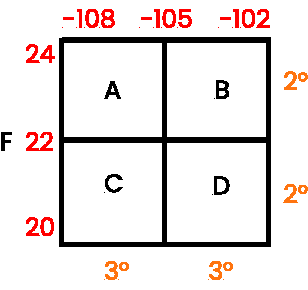
\includegraphics[width=0.5\textwidth]{sig11.pdf}
  \caption{Parámetros UTM, ej. -105-z13, False eastern: 500,000; False northern=0.0000 y latitud de oriden = $0^{\circ}$}
  \label{sig11}
\end{figure}
\begin{figure}[h!]
\centering
  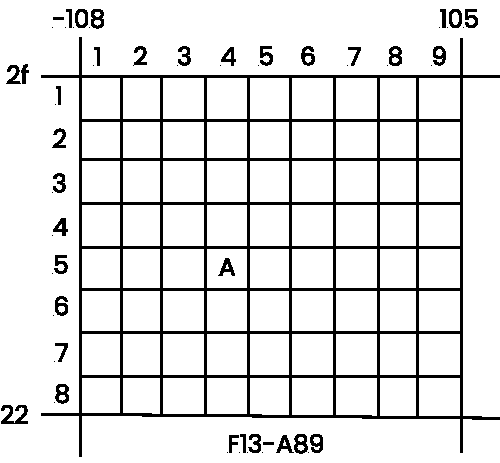
\includegraphics[width=0.5\textwidth]{sig12.pdf}
  \caption{Ejemplo de identificación de mapas bajo el sistema UTM}
  \label{sig12}
\end{figure}

Parámetros de la proyección Cónica:
False Eastern 2,500,000, false northern :0, Meridiano central: $-102^{\circ}$ y latitud de origen= $12^{\circ}$ PPrimer estándar 17.5 y Segundo estándar 29.5








%%%%%%%%%%%PÁGINA 37
\section{Cartografía Digital}
El término Sistema de Información Geográfica, SIG por sus siglas en español (en inglés GIS, Geographic Information System) se define como la ciencia y tecnología para el manejo integral de la información geográfica. El SIG está integrado por un conjunto de equipos electronico (hardware), de programas especializados (software), datos geograficos y tenicos, organizados para colectar, almacenar, actualizar, manipular, analizar y visualizar los datos georeferenciados para resolver problemas complejos de planeación y gestion. 

Son por tanto cuatro los elementos constitutivos de un sistema de estas características:

\begin{enumerate}
    \item Hardware
    \item Software
    \item Datos geográficos
    \item Equipo humano.
\end{enumerate}

Desde las décadas de los ochenta y noventa, el uso de los Sistemas de Información Geográfica, se ha venido generalizando, pasando del dominio de unos cuantos especialistas, a un gran número de usuarios tanto en el mundo de los negocios, universidades, organismos gubernamentales.  En la actualidad, diversas instituciones estàn invirtiendo grandes sumas de dinero en el desarrollo de base de datos georeferenciados.

La función de los SIG puede resumirse en seis puntos:

\begin{enumerate}
    \item Relacionar información de diferentes fuentes
    \item Capturar los datos 
    \item Integrar los datos
    \item Proyectar y registrar los datas
    \item Estructurar los datos
    \item Modelar los datos
\end{enumerate}

Las funciones especiales de los SIG consisten en los siguientes:

\begin{enumerate}
    \item Consulta y Desplegue de información
    \item Modelación topológica
    \item Redes
    \item Superposición
    \item Salida de datos
\end{enumerate}

\subsubsection{Modelo vector}

Una manera de representar los fenómenos geográficos es usando puntos, lineas y poligonos. Este modo de representación del mundo es generalmente llamado modelo de datos vectoriales, y es usado para representar y almacenar rasgos geográficos discretos tales come edificios, caminos, o límites de parcelas.

\begin{itemize}
    \item Los puntos son pares de coordenadas (V): los puntos tienen formas cero dimensional se usan para representar rasgos demasiados pequeños para ser defectados como líneas e áreas.
    \item Las líneas son definidas como una forma uni-dimensional demasiada estrecha para ser identificada como área. Las líneas son almacenadas como una serie de coordenadas x y ordenadas con atributos. El segmento de una linea puede ser rectal circular, eliprica o splined.
    \item Los poligonos son formas bidimensionales que representing tapos neograticos cumplies, y almacenados come na serie de segmentos que encierra un área.    
\end{itemize}
Otro tipo de datos vectoriales es la anotación. Son etiquetas descriptivas que son asociadas con los rasgos y despliegan nombres y atributos.

Las coordenadas son a menudo pares (x,y) o tripletes (x,y,z) donde z representa un valor como elevación o cualquier otro datos espaciales tales como contenido en sales, en contaminantes etc. 

Los datos vector usan una serie de posiciones para almacenar la información geográfica y

Existen tres objetos vectoriales básicos: puntos, lineas, políganos.

Estos objetos son llamados rasgos (features): 

\begin{itemize}
    \item Los rasgos Puntos (Point feature) son usados para representar objetos que no tienen dimensiones tales como pozos posición de muestreo etc.
    \item Los rasgas Líneas (Line features) representan objetas en una dimensión como carretera, ríos etc. 
    \item Los Poligonos (Polygon features) son usados para representar áreas en dos-dimensiones tal como parcelas, limites estatales etc.    
\end{itemize}
En cualquier caso, los rasgos o features son representados usando una o varias coordenadas x-y de posiciones. Un punto consiste de un solo par de coordenadas x-y, Una línea por dos a más pares de x-y, los puntos extremas de una linea son llamados NODES y los puntos intermediarios son llamados VERTEX,

El polígono es usado para representar una superficie bidimensional, tal como parcela, colonia, delegación política, municipio, estado etc., y son representados usando una serie de coordenadas x-y. El polígono puede ser definido como un grupo de vértices que delimiten una área.

El tipo de rasgos vectorial usado para representar un objeto depende de la escala del mapa.

\begin{figure}[h!]
\centering
  \includegraphics[width=0.5\textwidth]{sig2.pdf}
  \caption{Los rasgos (puntos, líneas o polígonos) son almacenados como una serie de coordenadas x-y dentro de un sistema de coordenadas rectangulares}
  \label{sig2}
\end{figure}

\subsubsection{Modelo Ráster}

En el modelo raster, el mundo se representa como una superficie que está dividida en grids regulares de celdas. Se requiere conocer las coordenadas de al menos una esquina del raster para poder localizarle en el espacio geográfico. 
El modelo raster es útil para almacenar y analizar los datos de las variables geográficas continuas dentro de un área. Cada celda contiene un valor que puede representar su membresía dentro de una clase o categoría, una medición o un valor interpretado.

Más pequeño es el tamaño de la celda del raster, más alto alta será la resolución espacial y más detallado será el mapa. Sin embargo, disminuyendo el tamaño de la celda para almacenar datos de mayor resolución incrementará en forma sustancial el volumen total de datos que se va tener que almacenar.

Los raster incluyen imágenes y grids. Las imágenes tales como fotografías aéreas escaneadas, imágenes de satélite, o mapa escaneado son usados para generar datos en el SIG. 

Los Grids son datos derivados y son a menudos usados para análisis y modelación. Pueden ser creadas a partir de muestras de puntos, tales como una superficie de concentraciones de sales. Los grids pueden ser creados convirtiendo datos vectoriales. Los grids almacenan valores continuos, tales como superficie de elevación.

Los grids pueden también almacenar categorías, tales como tipos de vegetación. Los grids que almacenan informaciones por categorías pueden almacenar atributos adicionales a cerca de cada categoría. Por ejemplo, un grid de tipos de vegetación puede almacenar, para cada categoría, un código numérico, el nombre del tipo de  vegetación, el nivel de aptitud del hábitat para ciertas especies de vida salvaje, y un tipo de código general.

\subsubsection{Modelo tin (triangulated irregular network model)}

En un modelo de red triangulado irregular, el mundo es representado como una red de triángulos ligados dibujados entre puntos irregularmente esparcidos con valores x, y, z. Los TINs son una manera eficiente de almacenar y analizar superficies. Las superficies heterogéneas que varias abruptamente en algunas áreas y menos en otras pueden ser modeladas más precisamente dentro de un volumen dado de datos, con una superficie triangulada que con un raster. Por eso se pondrá varios puntos en superficies con alta heterogeneidad, y menos puntos donde la superficie es menos variable.

\subsubsection{Estructura de los datos geograficos}

En ARCINFO y ARCVIEW, los datos geográficos están organizados por capas (layers) en base al tipo de rasgos geométricos (tipo de vector) usados para su representación (punto, linea o poligono). Cada uno de los rasgos por separado es clasificado  temáticamente (Fig.

El SIG permite trabajar a la vez con ambas partes de información: su forma perfectamente definida en plano y sus atributos temáticos asociados. Es decir, tiene que trabajar con cartografía y con bases de datos a la vez, uniendo ambas partes y constituyendo con todo ello una sola base de datos geográfica.

La construcción de una base de datos geográfica implica un proceso de simplificación cartografica  para pasar de la complejidad del mundo real a una representación simplificada. Este proceso de abstracción tiene diversos niveles comienza con la concepción de la estructura de la base de datos, generalmente en capas

Cada capa está asociada con una base de datos. El SIG permite trabajar con mapa y  base de datos en  forma simultanea. Esta capacidad de asociación de bases de datos temáticas junto con la descripción espacial precisa de objetos geográficos y las relaciones entre los mismos (topología) es lo que diferencia a un SIG de otros sistemas informáticos de gestión de información.

\section{GPS}

El sistema de posicionamiento global, GPS es un sistema de radio posicionamiento por navegación espacial conocido como NAVSTAR Navigation System by Timing And Ranging.

El GPS originalmente fueron diseñados para apoyar las operaciones militares dotando cada soldado y vehículos militares de receptores para proporcionar a cada uno de ellos:
\begin{itemize}
    \item La capacidad de geoposicionamiento autónoma, 24 horas al día con una precisión de 10 a 20 metros y una cobertura mundial, pudiendo funcionar bajo cualquier condición climatológica
    \item Actualmente sus aplicaciones no militares son amplias y diversas especialmente en sistemas de navegación aéreas, marítima y terrestre, en los levantamientos, y cartografías.
\end{itemize}
Desde la edad de la piedra hasta la edad espacial, los hombres han siempre encontrado un método de posicionamiento y de navegación. Las técnicas de posicionamiento usadas y la precisión de la misma han mejorado con el tiempo.

Algunas técnicas de navegación y de posicionamiento fueron: 
Recordar e identificar los objetos sobre el camino, las primeras coordenadas fueron determinadas por las estrellas.

En la edad de la radioseñal, multiplicando el tiempo de viaje de la señal por su velocidad, da la distancia entre el transmisor y el receptor de la señal. Siendo igual la velocidad de la señal a la velocidad de la luz, que es igual a 300,000Km/s, de la medición del tiempo dependerá la precisión en la medición:
\begin{equation}
    Distancia = Tiempo\times Velocidad
\end{equation}













